\documentclass[conference]{IEEEtran}
\IEEEoverridecommandlockouts
% Plantilla oficial IEEE conference (versión 06/27/2024). Compilar: pdflatex main; bibtex main; pdflatex main (x2)

\usepackage[utf8]{inputenc}
\usepackage[T1]{fontenc}
\usepackage[spanish,es-noshorthands,es-tabla]{babel}
\usepackage{cite}
\usepackage{amsmath,amssymb,amsfonts}
\usepackage{algorithm}
\usepackage{algorithmic}
\usepackage{graphicx}
\usepackage{textcomp}
\usepackage{xcolor}
\usepackage{booktabs}
\usepackage{enumitem}
\usepackage[hidelinks]{hyperref}
\setlist{leftmargin=*,itemsep=0pt,topsep=1pt,parsep=0pt}
\renewcommand{\algorithmicrequire}{\textbf{Entrada:}}
\floatname{algorithm}{Algoritmo}
\newcommand{\Dc}{\mathcal{D}}
\newcommand{\Lc}{\mathcal{L}}
\newcommand{\Bc}{\mathcal{B}}
\newcommand{\qq}{\textquestiondown}
\graphicspath{{figs/}}
\def\IEEEbibitemsep{0pt plus .5pt}

\begin{document}

\title{F-GAMR: Exploración guiada por lógica difusa y selección difusa del frente de Pareto para el enrutamiento multi-objetivo dinámico en redes SDN}

\author{\IEEEauthorblockN{Jesus Alonso Chaffe Gonzalez}
\IEEEauthorblockA{\textit{Rol USM: 202023501-5} --- IPD434 Seminario de Soft Computing\\
\textit{Departamento de Electrónica, Universidad Técnica Federico Santa María}, Valparaíso, Chile\\
Repositorio: \url{https://github.com/YizzHub/proyecto-ipd434-fgamr}}}

\maketitle

\begin{abstract}
Elegir rutas para muchas conexiones simultáneas exige equilibrar rapidez, pérdida de paquetes y congestión. GAMR (Tran \textit{et al.}, 2025) resuelve este problema en redes definidas por software (SDN) mediante búsqueda evolutiva y memoria de rutas. No obstante, parte de su exploración elige vecinos al azar y su selección final prioriza compartir menos enlaces, no directamente la calidad de servicio (QoS). Proponemos F-GAMR: dos sistemas de lógica difusa Mamdani, interpretables y sin entrenamiento. FIS-1 guía la construcción y modificación de rutas; FIS-2 selecciona un compromiso entre retardo y pérdida. Evaluamos la extensión en un simulador fluido sobre Oxford y Chinanet, con 30 semillas en la comparación principal y Wilcoxon pareado. Frente a GAMR, la pérdida realizada disminuye 2.8--6.1\% y el tiempo de cómputo 7.3--18.3\%. En Chinanet mejora también la calidad del conjunto de soluciones; en Oxford esa mejora no es significativa. La ablación separa ambos aportes y muestra que reducir pérdida puede exigir algo más de retardo.
\end{abstract}

\begin{IEEEkeywords}
SDN, enrutamiento multi-objetivo, NSGA-II, lógica difusa, Mamdani, calidad de servicio, hipervolumen.
\end{IEEEkeywords}

\section{Introducción}
Una videollamada necesita paquetes que lleguen a tiempo y con pocas pérdidas. Elegir el camino con menos saltos no garantiza ninguna de esas condiciones: varias conexiones pueden concentrarse en el mismo enlace y congestionar la red. En redes tradicionales, los equipos distribuyen las decisiones de reenvío; las redes definidas por software (SDN) separan ese reenvío del control y permiten programar rutas con una visión global~\cite{kreutz2015sdn}. Así pueden considerar calidad de servicio (QoS): retardo, pérdida y carga. Sin embargo, el enrutamiento sujeto a múltiples restricciones QoS es computacionalmente difícil~\cite{wang1996qos}, especialmente con solicitudes simultáneas y enlaces cambiantes.

GAMR~\cite{tran2025gamr} busca rutas conjuntamente con evolución y memoria. Nuestra réplica previa identificó dos oportunidades: sus caminatas y mutaciones eligen vecinos al azar, sin guía QoS; y el selector final prioriza menor solapamiento de enlaces, no directamente retardo ni pérdida.

El \textbf{objetivo general} es mejorar GAMR con conocimiento QoS interpretable: (P1) mejorar el conjunto de soluciones y reducir tiempo guiando la exploración; (P2) reducir pérdida realizada equilibrando retardo y pérdida. El \textbf{alcance} es simulación controlada, no despliegue real. Aportamos \textbf{FIS-1}, diez reglas para guiar construcción y mutación; \textbf{FIS-2}, seis reglas para elegir un compromiso; y una evaluación reproducible con ablación (componentes separados), calibración independiente y un diseño descartado.

\section{Marco teórico y trabajos relacionados}
\subsection{Redes definidas por software}
Una SDN distingue tres planos~\cite{kreutz2015sdn}: \emph{datos}, los switches que reenvían paquetes; \emph{control}, el controlador que obtiene mediciones y programa los switches; y \emph{aplicación}, donde se decide la política de enrutamiento. OpenFlow permite comunicar control y datos~\cite{mckeown2008openflow}. F-GAMR ocuparía el plano de aplicación: recibe el estado medido, calcula rutas y entrega una configuración al controlador. Aquí se simulan esos estados y rutas; no se ejecutan OpenFlow ni switches reales. La decisión debe terminar antes de que sus mediciones pierdan utilidad.

\subsection{Métricas de calidad de servicio}
El \emph{retardo} mide cuánto tarda un paquete: en una ruta $p_k$, $\Dc_k=\sum_{e\in p_k}delay_e$ [ms]. La \emph{pérdida} mide la fracción que no llega: $\Lc_k=1-\prod_{e\in p_k}(1-loss_e)$; se multiplica por 100 para expresarla en \%. Dos enlaces con pérdida 10\% producen 19\%, no 20\%. El \emph{ancho de banda disponible} [Mbps] lo limita el enlace con menor capacidad residual~\cite{tran2025gamr,wang1996qos}. La \emph{utilización} es $\rho_e=\text{carga}_e/bw_e$: 80\,Mbps sobre 100\,Mbps significa 80\%. Cerca de la saturación crece la espera y, con sobrecarga, el modelo descarta paquetes.

\subsection{Optimización multi-objetivo y NSGA-II}
Un \emph{algoritmo genético} (AG) mejora una población de soluciones combinándolas y modificándolas. Aquí cada individuo representa todas las rutas del intervalo, no una sola. NSGA-II~\cite{deb2002nsga2} busca varios objetivos: conserva soluciones que ninguna otra mejora simultáneamente en todos ellos y mantiene alternativas diversas. Esas soluciones forman el \emph{frente de Pareto}; por ejemplo, una puede ser más rápida y otra perder menos paquetes. El \textbf{hipervolumen} (HV)~\cite{zitzler1999hv} mide el volumen cubierto por el frente hasta un punto de referencia desfavorable (mayor es mejor). El \textbf{IGD}~\cite{coello2004igd} es la distancia media desde un frente de referencia a las soluciones encontradas (menor es mejor). Ambos evalúan el conjunto, no la ruta finalmente instalada.

\subsection{Lógica difusa}
La lógica difusa permite expresar ``retardo bajo'' o ``carga alta'' gradualmente, con pertenencia $\mu\in[0,1]$, en lugar de umbrales rígidos~\cite{zadeh1965fuzzy}. Ese grado no es una probabilidad. Un sistema de inferencia difusa (FIS) Mamdani~\cite{mamdani1975} combina reglas \emph{SI--ENTONCES}: usa mínimo para ``Y'', recorta cada salida al grado de activación, agrega por máximo y obtiene una puntuación numérica con el centroide (centro de área). La hibridación une dos técnicas del curso: búsqueda evolutiva para explorar y reglas difusas para aportar conocimiento interpretable.

\subsection{Trabajos relacionados}
GAMR~\cite{tran2025gamr} compara con evolutivos, Min-Hop y LCP-WAC (predictor LSTM). La hibridación genético-difusa suele adaptar parámetros~\cite{herrera2003fuzzyga}; la exploración sesgada por heurísticas aparece en colonias de hormigas~\cite{dorigo2004aco} y la memoria en evolución dinámica~\cite{nguyen2012dynamic}. F-GAMR usa reglas QoS \emph{dentro} de la construcción y selección de rutas, no para sintonizar parámetros.

\section{Problema y algoritmo base GAMR}
La red es un grafo $G=(\mathcal{V},\mathcal{E})$ de hosts $H$, servidores $S$ y switches $M$. En cada intervalo $t$ llegan $N_r$ solicitudes $R_k=(H_i,S_j,B_k)$: el host $H_i$ quiere conectarse al servidor $S_j$ con un ancho de banda $B_k$. Hay que encontrar un conjunto de rutas sin ciclos $\Phi^t=\{p_k\}$, una por solicitud, que minimice~\cite{tran2025gamr}:
\begin{equation}
f(\Phi^t)=\Big\{\tfrac{1}{N_r}\textstyle\sum_k \Dc_k,\ \tfrac{1}{N_r}\sum_k \Lc_k,\ f_3\Big\},\quad \text{s.a. } \Bc_k\ge B_k .\label{eq:obj}
\end{equation}
El paper define $f_3=1-\min_{e\in\mathcal{E}}\rho_e$, pero ese mínimo global resultó casi constante en la réplica: solo 3 valores distintos en una población. Usamos para todos los evolutivos la versión del código oficial: $f_3=\frac{1}{N_r}\sum_k\max_{e\in p_k}\min(\rho_e,1)$, promedio de la utilización del enlace más cargado de cada ruta, acotada a 100\%. $\Bc_k$ usa capacidad residual tras la carga de fondo; no garantiza por sí sola capacidad para todas las solicitudes juntas. Las configuraciones factibles tienen prioridad sobre las infactibles~\cite{deb2000constraint}.

GAMR procede así: (1) construye una población de $N=100$ configuraciones; para cada ruta reutiliza memoria (PSBI) con probabilidad $\alpha=0.5$ o realiza una caminata aleatoria con retroceso (RSBI); (2) cruza rutas en un nodo común ($p_c=0.8$), inserta vecinos por mutación ($p_m=0.1$) y elimina ciclos; (3) selecciona con NSGA-II; (4) termina la búsqueda del intervalo si $|HV_G-HV_{G-10}|<10^{-4}$ o alcanza 500 generaciones; (5) instala la configuración con menor solapamiento y guarda una ruta por servidor (memoria PRSM). \textbf{Detenerse no interrumpe el tráfico}: termina el cálculo, se usan las rutas elegidas y se vuelve a optimizar en el siguiente intervalo. No certifica un óptimo global; IGD se usa para evaluar, no para parar.

\section{Método propuesto: F-GAMR}
F-GAMR conserva intactos la memoria, $\alpha$, el cruce, la selección y la parada de GAMR. Solo reemplaza dos elementos: la elección uniforme de vecinos (por FIS-1) y el criterio de instalación (por FIS-2).

\subsection{FIS-1: deseabilidad QoS de un salto}
Considere un salto $u\to v$ dentro de una ruta hacia el servidor $S$. FIS-1 recibe cuatro entradas en $[0,1]$, calculadas con el estado \emph{medido} del intervalo:
\begin{equation}
\begin{aligned}
\pi_{uv}&=\tfrac12\big(h_S(u)-h_S(v)+1\big), & c_e&=bg_e^t/bw_e^t,\\
d_e&=delay_e/(100\ \mathrm{ms}), & l_e&=loss_e/(10\ \%).
\end{aligned}
\end{equation}
El \emph{progreso} $\pi_{uv}$ usa $h_S(\cdot)$, los saltos hasta $S$: vale 1 si acerca al servidor, 1/2 si mantiene distancia y 0 si aleja. $d_e$ y $l_e$ normalizan el retardo y la pérdida por 100\,ms y 10\%~\cite{tran2025gamr}; $c_e$ mide la carga de fondo relativa a la capacidad. Diez reglas Mamdani producen la deseabilidad $w_{uv}\in[0,1]$; por ejemplo, ``SI acerca Y retardo bajo Y pérdida baja ENTONCES muy alta'' y ``SI carga alta ENTONCES baja'' (Fig.~\ref{fig:fis}a). La caminata elige el siguiente nodo mediante:
\begin{equation}
P(v\mid u)=\frac{w_{uv}^{\kappa}+\varepsilon}{\sum_{v'\in\mathcal{N}(u)\setminus\mathrm{vis}}\big(w_{uv'}^{\kappa}+\varepsilon\big)},\qquad \kappa=2,\ \varepsilon=0.01 .\label{eq:ruleta}
\end{equation}
Se mantiene el retroceso de RSBI y, como $\varepsilon>0$, ningún salto válido queda prohibido: la exploración se sesga hacia rutas prometedoras sin convertirse en un Dijkstra determinista. En la mutación, el nodo a insertar $\tilde\lambda$ entre $\lambda_1$ y $\lambda_2$ se elige con probabilidad $\propto q(\lambda_1,\tilde\lambda)\,q(\tilde\lambda,\lambda_2)$, donde $q$ es la deseabilidad con progreso neutro ($\pi=\tfrac12$).

\subsection{FIS-2: selector de compromiso}
Para cada solución $\Phi$ del frente final $F^1$, FIS-2 recibe su retardo medio $\hat{\Dc}$ y su pérdida media $\hat{\Lc}$, ambos normalizados min--max \emph{dentro del frente}, de modo que el selector no depende de la escala de la instancia. Seis reglas expresan el compromiso: ambos bajos $\to$ aptitud muy alta; uno bajo y el otro medio $\to$ alta; ambos medios $\to$ media; cualquiera alto $\to$ baja (Fig.~\ref{fig:fis}b). Se instala $\Phi^\star=\arg\max_{\Phi\in F^1}\text{FIS-2}(\hat{\Dc},\hat{\Lc})$, con empates resueltos por menor retardo. El Algoritmo~\ref{alg:fgamr} resume el método.

\begin{figure}[t]
\centering
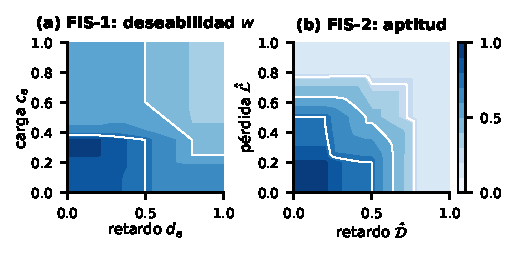
\includegraphics[width=\columnwidth]{fis.pdf}
\caption{Superficies de decisión. (a) FIS-1: deseabilidad de un salto que acerca al servidor (pérdida 2\%), según el retardo y la carga. (b) FIS-2: aptitud según el retardo y la pérdida normalizados dentro del frente.}
\label{fig:fis}
\end{figure}

\begin{algorithm}[t]
\caption{F-GAMR en el intervalo $t$ (en \textbf{negrita}, lo nuevo respecto de GAMR)}\label{alg:fgamr}
\begin{algorithmic}[1]
\REQUIRE estado medido $\Delta^t$, solicitudes $R^t$, memoria $\mathcal{M}$
\STATE \textbf{FIS-1: calcular $w_{uv}$ para todo salto $(u,v,S)$ y $q_e$}
\STATE $P\leftarrow$ por solicitud: PSBI($\mathcal{M}$) si $U[0,1]\le\alpha$; si no, \textbf{RSBI guiada}~\eqref{eq:ruleta}
\REPEAT
\STATE $O\leftarrow$ cruce + \textbf{mutación guiada} + eliminación de ciclos
\STATE $P\leftarrow$ selección NSGA-II$(P\cup O)$; registrar $HV_G$
\UNTIL{$(G\ge10\ \AND\ |HV_G-HV_{G-10}|<10^{-4})$ \OR $G=G^{\max}$}
\STATE $\Phi^\star\leftarrow$ \textbf{$\arg\max$ FIS-2 sobre $F^1$}; instalar; actualizar $\mathcal{M}$
\end{algorithmic}
\end{algorithm}

\textbf{Costo.} FIS-1 precalcula puntuaciones una vez por intervalo, con costo $\mathcal{O}(N_s|\mathcal{E}|)$; la ruleta recorre los vecinos y FIS-2 puntúa el frente una vez. No cambia el orden de complejidad de la búsqueda.

\textbf{Calibración.} Usamos semillas 500--503, distintas de evaluación (0--29). Adaptar $\alpha$ e inyectar individuos según volatilidad dio resultados inconsistentes (tiempo hasta $+72\%$; HV $-19\%$ con $\alpha\to0.8$) y se descartó. $\kappa=2$ mejoró HV 3.7--14.3\% en validación; $\kappa=4$ perdió diversidad. Añadir entradas a FIS-2 no mejoró QoS.

\section{Diseño experimental}
\textbf{Simulador.} Se reemplaza Mininet + Ryu~\cite{tran2025gamr} por un modelo fluido Python: representa demandas y capacidad, no paquetes individuales. Usa Oxford (20 switches, 26 enlaces) y Chinanet (42, 66), del Internet Topology Zoo~\cite{knight2011zoo}. Los enlaces tienen retardo $U[5,100]$\,ms, pérdida en $\{0.1,0.5,1,2,3,4,5,7,9,10\}\%$ y capacidad base $U[30,200]$\,Mbps~\cite{tran2025gamr}. $\beta$ controla perturbaciones hasta $\pm\beta$ de esa capacidad. Con $\beta=0$ se asigna la misma capacidad fija a todos los enlaces; la carga de fondo sí cambia, por lo que no es una red completamente estática. Por intervalo, $bg_e\sim U[0,0.3]bw_e$ y cada solicitud demanda $U[0.5,3]$\,Mbps. La carga total determina $\rho_e$; la cola añade $10\min(\rho_e/(1-\rho_e),20)$\,ms si $\rho_e<1$ (200\,ms si $\rho_e\ge1$), y el desborde añade pérdida $\max(0,1-1/\rho_e)$.

\textbf{Experimentos} ($N_s=2$ servidores, para que haya congestión). \textbf{E1} (comparación principal y ablación): Oxford y Chinanet, $N_r=50$, $\beta\in\{5,55\}\%$, 30 semillas. \textbf{E2} (escalabilidad): Oxford, $N_r\in\{10,20,50,100\}$, $\beta=20\%$, 10 semillas. \textbf{E3} (robustez al desorden): Chinanet, $N_r=100$, $\beta\in\{0,5,20,55\}\%$, 10 semillas.

\textbf{Líneas base.} \emph{Min-Hop}: mínimos saltos; \emph{QoS-Dijkstra}: mínimo retardo con capacidad residual $\ge B_k$, por solicitud separada; \emph{NSGA-II}: operadores de GAMR sin memoria ($\alpha=0$); y \emph{GAMR}. E3 añade \emph{LCP-WAC*}, proxy de costo ponderado con predicción histórica, sin LSTM. La ablación evalúa solo FIS-1 y solo FIS-2. Todos los evolutivos usan $N=100$, máximo 500 generaciones, $p_c=0.8$, $p_m=0.1$ y torneo binario~\cite{tran2025gamr}.

\textbf{Protocolo.} Cada semilla es una secuencia de 4 intervalos. En cada uno llegan solicitudes nuevas y \emph{todos} los algoritmos resuelven la misma instancia. Después, las rutas se instalan, la red evoluciona a $\Delta^{t+1}$ y la QoS se mide en ese estado \emph{realizado}, no en el que se optimizó. El intervalo 1 (memoria vacía) se descarta y se promedian los intervalos 2--4: una observación por semilla.

\textbf{Métricas.} \emph{Frente}: HV con referencia $r=(1,1,1)$ e IGD frente a los no dominados de la unión de resultados, una referencia empírica, no el óptimo verdadero. Los objetivos se normalizan con una escala conjunta por instancia. \emph{Costo}: tiempo por configuración completa [s], no por paquete. \emph{QoS realizada}: retardo [ms], pérdida [\%], máxima utilización acotada a 100\% y solicitudes sin enlaces sobrecargados [\%]. Se informa media $\pm$ desviación estándar entre semillas; no es un intervalo de confianza. Wilcoxon~\cite{wilcoxon1945} compara pares por semilla ($p<0.05$, sin corrección por comparaciones múltiples). Las mejoras porcentuales son relativas: pasar de 10.77\% a 10.11\% de pérdida reduce 0.66 puntos porcentuales, o 6.1\% respecto del valor inicial.

\begin{table*}[!t]
\centering
\caption{E1 --- Calidad del frente de Pareto y tiempo de c\'omputo por instancia ($N_s{=}2$, $N_r{=}50$; media$\pm$desv.\ est.\ sobre 30 semillas). HV$\uparrow$, IGD$\downarrow$, t$\downarrow$. \textbf{Negrita}: mejor; $^\dagger$: diferencia con GAMR significativa (Wilcoxon pareado, $p<0.05$).}
\label{tab:e1moo}
\scriptsize
\setlength{\tabcolsep}{2.2pt}
\begin{tabular}{l|ccc|ccc|ccc|ccc}
\toprule
 & \multicolumn{3}{c|}{Oxford, $\beta{=}5\%$} & \multicolumn{3}{c|}{Oxford, $\beta{=}55\%$} & \multicolumn{3}{c|}{Chinanet, $\beta{=}5\%$} & \multicolumn{3}{c}{Chinanet, $\beta{=}55\%$} \\
Algoritmo & HV & IGD & t [s] & HV & IGD & t [s] & HV & IGD & t [s] & HV & IGD & t [s] \\
\midrule
NSGA-II & 0.622{\tiny$\pm$0.072}$^\dagger$ & 0.094{\tiny$\pm$0.037}$^\dagger$ & 6.98{\tiny$\pm$1.21}$^\dagger$ & 0.635{\tiny$\pm$0.060}$^\dagger$ & 0.090{\tiny$\pm$0.032}$^\dagger$ & 6.93{\tiny$\pm$1.10}$^\dagger$ & 0.669{\tiny$\pm$0.069} & 0.087{\tiny$\pm$0.035} & 9.11{\tiny$\pm$1.84}$^\dagger$ & 0.675{\tiny$\pm$0.054} & 0.080{\tiny$\pm$0.028} & 9.50{\tiny$\pm$1.75}$^\dagger$ \\
GAMR & 0.687{\tiny$\pm$0.061} & 0.060{\tiny$\pm$0.023} & 6.14{\tiny$\pm$1.58} & 0.694{\tiny$\pm$0.066} & 0.059{\tiny$\pm$0.017} & 6.05{\tiny$\pm$1.40} & 0.679{\tiny$\pm$0.060} & 0.081{\tiny$\pm$0.026} & 7.44{\tiny$\pm$1.69} & 0.678{\tiny$\pm$0.048} & 0.077{\tiny$\pm$0.016} & 7.68{\tiny$\pm$1.70} \\
\midrule
solo FIS-1 & 0.695{\tiny$\pm$0.070} & 0.066{\tiny$\pm$0.026} & \textbf{5.01}{\tiny$\pm$1.43}$^\dagger$ & 0.688{\tiny$\pm$0.062} & 0.066{\tiny$\pm$0.021} & \textbf{4.88}{\tiny$\pm$1.12}$^\dagger$ & 0.729{\tiny$\pm$0.049}$^\dagger$ & \textbf{0.057}{\tiny$\pm$0.015}$^\dagger$ & \textbf{6.56}{\tiny$\pm$1.78}$^\dagger$ & 0.720{\tiny$\pm$0.035}$^\dagger$ & 0.064{\tiny$\pm$0.023}$^\dagger$ & \textbf{6.83}{\tiny$\pm$1.56}$^\dagger$ \\
solo FIS-2 & 0.690{\tiny$\pm$0.065} & \textbf{0.054}{\tiny$\pm$0.015} & 6.23{\tiny$\pm$1.43} & 0.693{\tiny$\pm$0.059} & \textbf{0.057}{\tiny$\pm$0.018} & 6.11{\tiny$\pm$1.20} & 0.691{\tiny$\pm$0.046} & 0.074{\tiny$\pm$0.026} & 7.83{\tiny$\pm$1.74} & 0.672{\tiny$\pm$0.049} & 0.081{\tiny$\pm$0.031} & 7.82{\tiny$\pm$1.54} \\
\textbf{F-GAMR} & \textbf{0.697}{\tiny$\pm$0.073} & 0.067{\tiny$\pm$0.026} & 5.12{\tiny$\pm$1.31}$^\dagger$ & \textbf{0.698}{\tiny$\pm$0.065} & 0.063{\tiny$\pm$0.028} & 4.94{\tiny$\pm$1.26}$^\dagger$ & \textbf{0.734}{\tiny$\pm$0.055}$^\dagger$ & 0.061{\tiny$\pm$0.021}$^\dagger$ & 6.87{\tiny$\pm$1.67}$^\dagger$ & \textbf{0.724}{\tiny$\pm$0.046}$^\dagger$ & \textbf{0.062}{\tiny$\pm$0.024}$^\dagger$ & 7.13{\tiny$\pm$1.83}$^\dagger$ \\
\bottomrule
\end{tabular}
\end{table*}

\begin{figure*}[t]
\centering
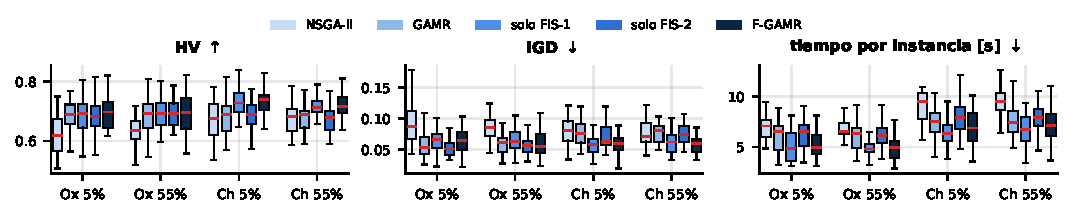
\includegraphics[width=\textwidth]{e1_moo.pdf}
\caption{E1: distribución sobre 30 semillas de HV, IGD y tiempo (Ox/Ch = Oxford/Chinanet; \% = desorden $\beta$). Cajas: rango intercuartílico; línea roja: mediana.}
\label{fig:e1}
\end{figure*}

\begin{table*}[!t]
\centering
\caption{E1 --- QoS medida en el estado realizado de la red $\Delta^{t+1}$ (media$\pm$desv.\ est., 30 semillas; todas las m\'etricas $\downarrow$). \textbf{Negrita}: mejor; $^\dagger$: $p<0.05$ frente a GAMR.}
\label{tab:e1qos}
\scriptsize
\setlength{\tabcolsep}{2.2pt}
\begin{tabular}{l|ccc|ccc|ccc|ccc}
\toprule
 & \multicolumn{3}{c|}{Oxford, $\beta{=}5\%$} & \multicolumn{3}{c|}{Oxford, $\beta{=}55\%$} & \multicolumn{3}{c|}{Chinanet, $\beta{=}5\%$} & \multicolumn{3}{c}{Chinanet, $\beta{=}55\%$} \\
Algoritmo & Ret.\,[ms] & P\'erd.\,[\%] & $\rho_{\max}$[\%] & Ret.\,[ms] & P\'erd.\,[\%] & $\rho_{\max}$[\%] & Ret.\,[ms] & P\'erd.\,[\%] & $\rho_{\max}$[\%] & Ret.\,[ms] & P\'erd.\,[\%] & $\rho_{\max}$[\%] \\
\midrule
MH & 224.8{\tiny$\pm$58.9}$^\dagger$ & 14.40{\tiny$\pm$5.03} & 77.4{\tiny$\pm$14.8}$^\dagger$ & 239.6{\tiny$\pm$61.4}$^\dagger$ & 16.20{\tiny$\pm$6.93}$^\dagger$ & 83.3{\tiny$\pm$12.4}$^\dagger$ & 169.7{\tiny$\pm$47.6}$^\dagger$ & 11.33{\tiny$\pm$4.07}$^\dagger$ & 68.3{\tiny$\pm$19.1}$^\dagger$ & 179.1{\tiny$\pm$55.0}$^\dagger$ & 11.83{\tiny$\pm$4.07}$^\dagger$ & 73.3{\tiny$\pm$17.2}$^\dagger$ \\
QoS-Dijkstra & 231.6{\tiny$\pm$79.9}$^\dagger$ & 16.19{\tiny$\pm$6.58}$^\dagger$ & 79.1{\tiny$\pm$14.9}$^\dagger$ & 247.4{\tiny$\pm$81.5}$^\dagger$ & 18.50{\tiny$\pm$7.64}$^\dagger$ & 84.9{\tiny$\pm$12.4}$^\dagger$ & 184.1{\tiny$\pm$45.2} & 16.00{\tiny$\pm$8.16}$^\dagger$ & 81.6{\tiny$\pm$17.3}$^\dagger$ & 203.3{\tiny$\pm$59.9}$^\dagger$ & 17.60{\tiny$\pm$7.64}$^\dagger$ & 84.4{\tiny$\pm$17.0}$^\dagger$ \\
\midrule
NSGA-II & 199.6{\tiny$\pm$41.6}$^\dagger$ & 12.91{\tiny$\pm$3.51} & \textbf{65.4}{\tiny$\pm$9.1}$^\dagger$ & 219.5{\tiny$\pm$54.8}$^\dagger$ & 13.38{\tiny$\pm$3.75} & \textbf{75.8}{\tiny$\pm$12.1} & 166.9{\tiny$\pm$45.6} & 10.80{\tiny$\pm$3.88} & 65.7{\tiny$\pm$20.1} & 177.2{\tiny$\pm$54.0}$^\dagger$ & 11.35{\tiny$\pm$3.96} & 70.3{\tiny$\pm$18.5} \\
GAMR & \textbf{196.3}{\tiny$\pm$41.2} & 12.85{\tiny$\pm$3.45} & 66.6{\tiny$\pm$9.4} & 216.7{\tiny$\pm$54.3} & 13.34{\tiny$\pm$3.79} & 76.1{\tiny$\pm$11.8} & 166.5{\tiny$\pm$45.5} & 10.77{\tiny$\pm$3.92} & 65.2{\tiny$\pm$20.4} & 174.3{\tiny$\pm$53.2} & 11.26{\tiny$\pm$3.99} & \textbf{69.9}{\tiny$\pm$18.6} \\
\midrule
solo FIS-1 & 197.5{\tiny$\pm$43.3} & 12.81{\tiny$\pm$3.41} & 67.5{\tiny$\pm$9.9} & \textbf{216.6}{\tiny$\pm$54.9} & 13.41{\tiny$\pm$3.96} & 76.4{\tiny$\pm$11.8} & \textbf{164.5}{\tiny$\pm$45.6}$^\dagger$ & 10.82{\tiny$\pm$3.92} & \textbf{64.9}{\tiny$\pm$20.5} & \textbf{173.5}{\tiny$\pm$52.6} & 11.24{\tiny$\pm$3.98} & 70.3{\tiny$\pm$18.4} \\
solo FIS-2 & 198.6{\tiny$\pm$42.7}$^\dagger$ & 12.50{\tiny$\pm$3.54}$^\dagger$ & 66.9{\tiny$\pm$8.9} & 218.3{\tiny$\pm$53.8} & 13.10{\tiny$\pm$3.89} & 75.8{\tiny$\pm$11.6} & 168.4{\tiny$\pm$47.4}$^\dagger$ & 10.14{\tiny$\pm$4.02}$^\dagger$ & 67.2{\tiny$\pm$19.1}$^\dagger$ & 178.2{\tiny$\pm$53.6}$^\dagger$ & 10.68{\tiny$\pm$4.03}$^\dagger$ & 71.9{\tiny$\pm$17.1}$^\dagger$ \\
\textbf{F-GAMR} & 198.9{\tiny$\pm$42.4}$^\dagger$ & \textbf{12.38}{\tiny$\pm$3.56}$^\dagger$ & 68.2{\tiny$\pm$8.9}$^\dagger$ & 220.3{\tiny$\pm$55.0} & \textbf{12.97}{\tiny$\pm$3.90}$^\dagger$ & 77.0{\tiny$\pm$11.7} & 166.9{\tiny$\pm$47.3} & \textbf{10.11}{\tiny$\pm$4.01}$^\dagger$ & 67.8{\tiny$\pm$18.8}$^\dagger$ & 176.3{\tiny$\pm$53.9} & \textbf{10.66}{\tiny$\pm$4.09}$^\dagger$ & 72.5{\tiny$\pm$16.8}$^\dagger$ \\
\bottomrule
\end{tabular}
\end{table*}

\section{Resultados}
\subsection{E1: calidad del frente y tiempo (P1)}
La Tabla~\ref{tab:e1moo} y la Fig.~\ref{fig:e1} resumen estos resultados. En \textbf{Chinanet}, F-GAMR eleva el HV de GAMR de 0.679 a 0.734 con $\beta=5\%$ ($+8.2\%$, $p=2\times10^{-8}$) y de 0.678 a 0.724 con $\beta=55\%$ ($+6.8\%$), y reduce el IGD entre 20\% y 25\% ($p<10^{-3}$). En \textbf{Oxford}, las diferencias de HV e IGD no son significativas ($p>0.2$). En ambas topologías F-GAMR \textbf{converge antes}: en Oxford necesita unas 50 generaciones frente a 62 de GAMR y su tiempo baja entre 16.7\% y 18.3\% ($p<10^{-4}$); en Chinanet baja entre 7.3\% y 7.7\% ($p<0.03$). \textbf{Frente a NSGA-II}, F-GAMR mejora el HV entre 7\% y 12\%, el IGD entre 22\% y 30\% y el tiempo entre 25\% y 29\% ($p<0.005$).

\textbf{Ablación.} La mejora de HV, IGD y tiempo proviene de FIS-1: por sí solo sube el HV de Chinanet entre 6\% y 7\% y recorta el tiempo entre 11\% y 19\% ($p<0.002$). FIS-2 solo no altera el frente (todas sus diferencias tienen $p>0.07$), lo esperado porque actúa después de la evolución.

\subsection{E1: QoS realizada y selección final (P2)}
La Tabla~\ref{tab:e1qos} muestra la QoS medida. F-GAMR obtiene la \textbf{menor pérdida} en los cuatro escenarios: entre 2.8\% y 6.1\% menos que GAMR (p.\,ej., 10.11\% frente a 10.77\% en Chinanet con $\beta=5\%$; $p\le10^{-4}$). El costo en \textbf{retardo} es pequeño, entre $+0.3$\% y $+1.6$\%, y solo es significativo en Oxford con $\beta=5\%$ ($p=0.025$). Frente a \textbf{Min-Hop}, F-GAMR reduce la pérdida entre 10\% y 20\% y el retardo hasta 11.5\%. \textbf{QoS-Dijkstra}, al optimizar cada solicitud de forma egoísta, satura los mismos enlaces y obtiene la peor pérdida (16--18.5\%) y la mayor $\rho_{\max}$. La ablación atribuye la reducción de pérdida a FIS-2: solo FIS-1 no cambia la pérdida.

\textbf{Criterios de selección.} Para aislar FIS-2 aplicamos cuatro criterios sobre \emph{los mismos} frentes de GAMR (Fig.~\ref{fig:res}d). \emph{Mínimo retardo} reduce retardo 1.3--2.3\%, pero aumenta pérdida 2.1--3.3\%. \emph{FIS-2} reduce pérdida 1.4--6.1\% ($p<0.03$) a cambio de 0.9--2.5\% más retardo. Frente al \emph{punto rodilla} (aquí, solución más cercana al ideal normalizado), obtiene medias realizadas menores en ambas métricas en tres escenarios. Esto no implica dominar esas soluciones en el frente de tres objetivos.

\begin{figure*}[t]
\centering
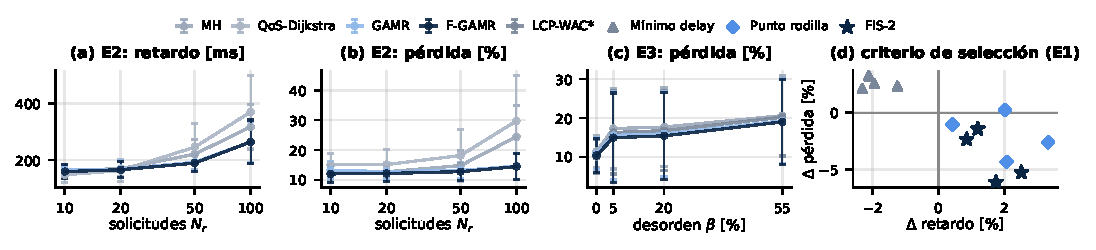
\includegraphics[width=\textwidth]{resultados.pdf}
\caption{(a,b) E2: retardo y pérdida en Oxford según el número de solicitudes simultáneas $N_r$ (media$\pm$desv.\ est., 10 semillas). (c) E3: pérdida en Chinanet según el desorden $\beta$. (d) QoS realizada de cada criterio aplicado a los mismos frentes de GAMR, en $\Delta$\% frente a ``menor solapamiento'' (un punto por escenario de E1; el cuadrante inferior izquierdo es mejor en ambas métricas).}
\label{fig:res}
\end{figure*}

\subsection{E2 y E3: escalabilidad y desorden de la red}
\textbf{Escalabilidad (Fig.~\ref{fig:res}a,b).} Con $N_r=100$ las heurísticas se degradan: Min-Hop alcanza 316.7\,ms y 24.5\% de pérdida, y QoS-Dijkstra 368.8\,ms y 29.7\%, frente a unos 264\,ms y 14.5\% en los evolutivos. F-GAMR reduce pérdida respecto de GAMR 8.9\%, 5.1\% y 3.0\% para 10, 20 y 50 solicitudes ($p<0.01$); con 100, el 1.0\% no es significativo. El tiempo baja 12--19\% ($p<0.05$), pero con 100 solicitudes aún requiere 10.52\,s por configuración, frente a 12.92\,s de GAMR: no demuestra operación en tiempo real.

\textbf{Desorden (Fig.~\ref{fig:res}c).} Con $\beta=0$, LCP-WAC* obtiene las menores medias de retardo y pérdida (189.7\,ms; 10.12\%). Su predicción de capacidad es exacta en ese caso, no la de carga de fondo. Para $\beta\ge5\%$, F-GAMR obtiene menores medias de pérdida (14.95--18.99\% frente a 16.26--20.21\%), pero la comparación con el proxy no demuestra significancia. Frente a GAMR reduce pérdida 3.2--4.4\% para $\beta\le20\%$ ($p=0.002$); con $\beta=55\%$, el 1.4\% no es significativo.

\section{Discusión crítica}
\textbf{Por qué funciona.} FIS-1 concentra la población inicial en rutas QoS-prometedoras sin anular el azar: en 2000 caminatas de una instancia de Oxford, la ruta inicial media pasó de 541 a 485\,ms y su pérdida de 45\% a 36\%. El HV arranca más alto y la parada por estancamiento se activa antes, lo que explica el ahorro de tiempo. FIS-2 sustituye un criterio topológico por uno de QoS. Ambos son complementarios: FIS-1 mejora el frente y el tiempo; FIS-2, la ruta instalada.

\textbf{Casos de fallo.} Oxford tiene pocas alternativas (grado medio 2.6, tres triángulos): la guía reduce rutas iniciales distintas de 36 a 22 en la demostración y el IGD empeora 8--12\%, sin significancia. Esto sugiere pérdida de diversidad, no prueba causal general. En E3, con $\beta=55\%$, la ventaja deja de ser significativa: las mediciones usadas al elegir pueden quedar obsoletas. FIS-2 también sube $\rho_{\max}$ 1--3 puntos al priorizar pérdida sobre solapamiento. El control adaptativo descartado concentraba rutas memorizadas; la mutación por inserción añadía desvíos.

\textbf{Limitaciones.} El modelo fluido no valida TCP/OpenFlow ni permite trasladar magnitudes al paper; LCP-WAC* no reproduce su LSTM. $\beta=0$ cambia también la homogeneidad de capacidades, no solo su variación temporal. Solo hay dos topologías y cuatro semillas de calibración; las pruebas múltiples sin ajuste aumentan el riesgo de falsos positivos. FIS-2 depende de las alternativas disponibles y no garantiza QoS futura. El ahorro es relativo, no prueba de tiempo real.

\section{Conclusiones y trabajo futuro}
La lógica difusa incorpora conocimiento QoS interpretable sin entrenamiento. \textbf{P1}: mejora el frente en Chinanet y reduce tiempo; no mejora significativamente el frente en Oxford. \textbf{P2}: F-GAMR reduce pérdida realizada 2.8--6.1\% en E1 con menos de 2\% de costo en retardo; la ablación atribuye ese aporte al selector. No es una mejora universal. Como trabajo futuro: validar en Mininet con TCP, ampliar topologías, adaptar $\kappa$ para preservar diversidad y ajustar pertenencias mediante evolución.

\textbf{Reproducibilidad.} El paquete del repositorio enlazado en la primera página contiene código, topologías, resultados crudos y notebook. El README documenta instalación y reproducción; \path{run_reproduction.py --solo-reporte} regenera el análisis y \path{scripts/informe_assets.py} las figuras del informe. Debe comprobarse acceso público al enlace antes de entregar.

\bibliographystyle{IEEEtran}
\bibliography{references}

\end{document}
